\newprob{1717152938}
{
    % 四模q18
    一列直線水波如圖射向圓弧形的障礙物。\\A series of wave is about to hit the obstacle as shown below.
    \par{\par\centering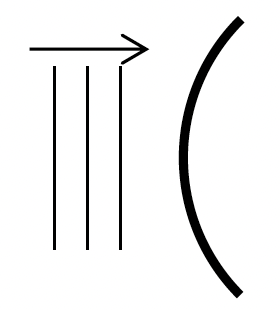
\includegraphics[width=.2\textwidth]{./img/ch2_weekend_mc_2024-05-31-18-55-50.png}\par}
    以下何者最能顯示反射後的水波?\\Which of the following best indicates the reflected wave?
    \begin{tasks}(2)
        \task \topalign{\par\centering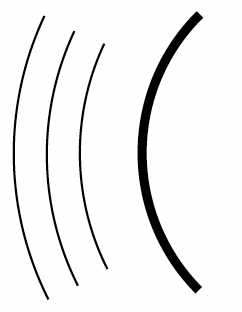
\includegraphics[width=.15\textwidth]{./img/ch2_weekend_mc_2024-05-31-18-57-35.png}\par}
        \task \topalign{\par\centering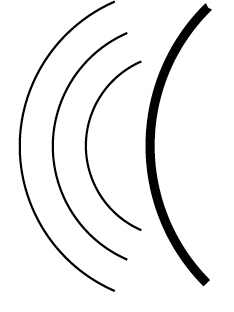
\includegraphics[width=.15\textwidth]{./img/ch2_weekend_mc_2024-05-31-18-57-48.png}\par}
        \task \topalign{\par\centering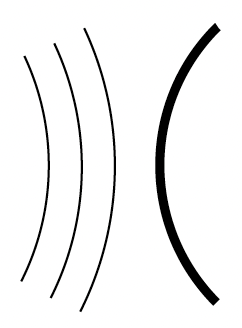
\includegraphics[width=.15\textwidth]{./img/ch2_weekend_mc_2024-05-31-18-57-23.png}\par}
        \task \topalign{\par\centering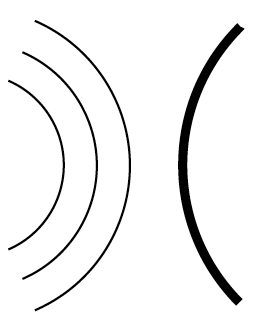
\includegraphics[width=.15\textwidth]{./img/ch2_weekend_mc_2024-05-31-18-57-09.png}\par}
    \end{tasks}
}{B}




\newprob{1717151247}
{


    % 一模MC Q17
    一列水波由淺水區進入深水區。\\ A series of water wave enters deep water region from shallow water region.
    % \par{\par\centering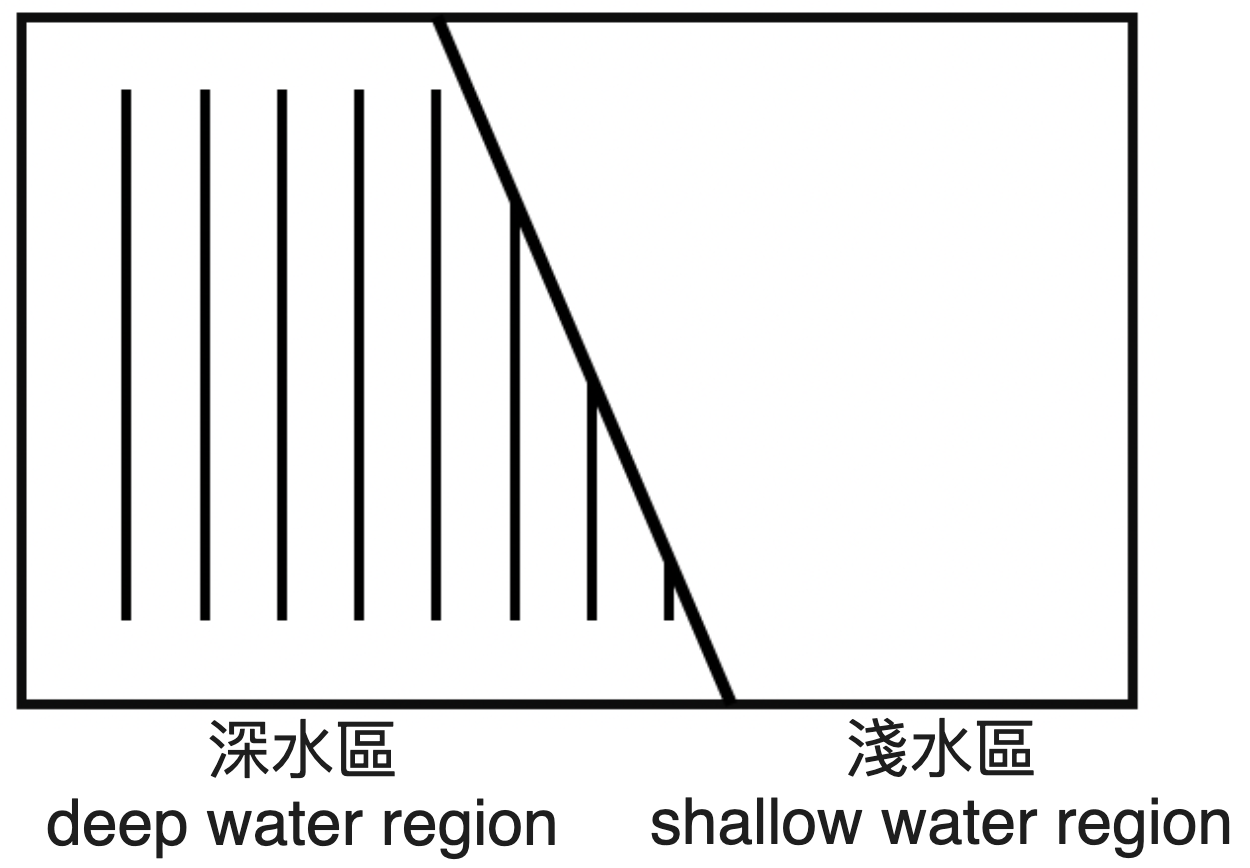
\includegraphics[width=\textwidth]{./img/ch2_weekend_mc_2024-05-31-18-32-55.png}\par}
    \par{\par\centering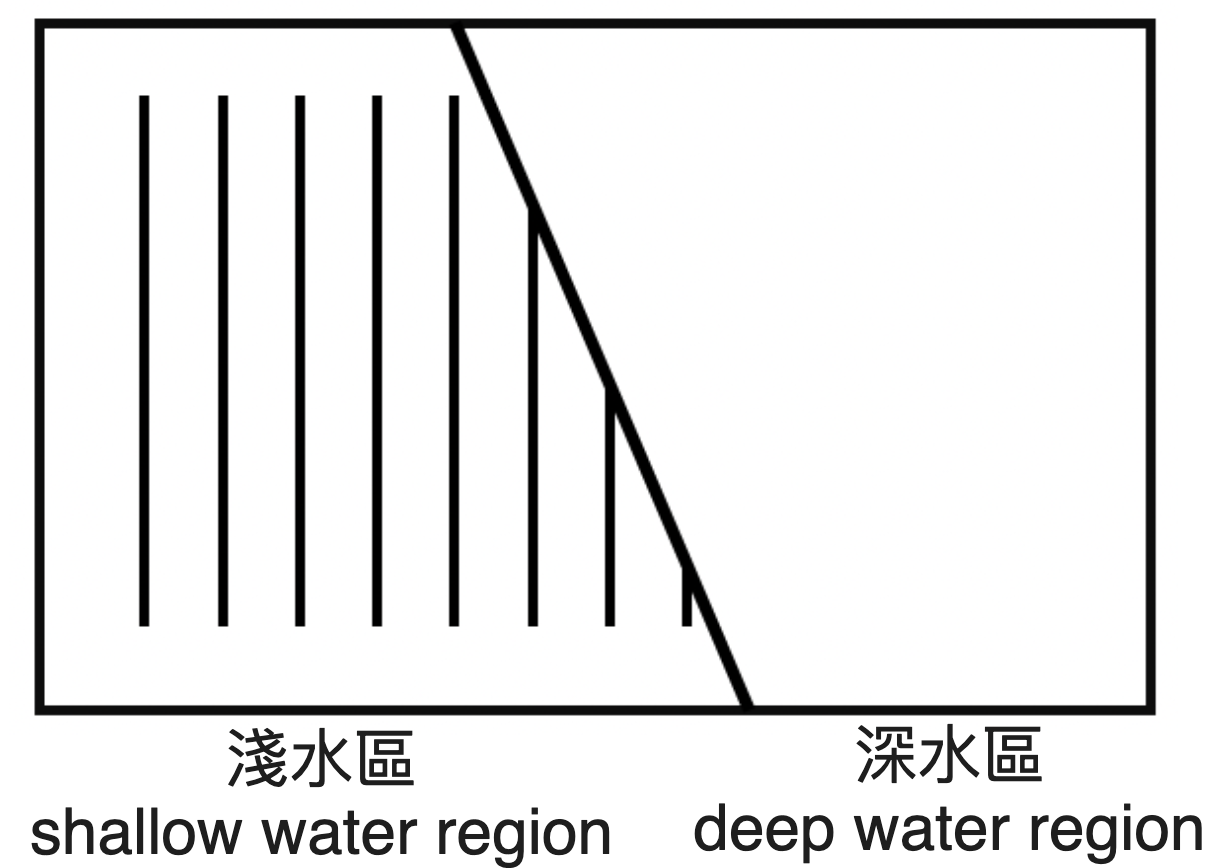
\includegraphics[width=.4\textwidth]{./img/ch2_weekend_mc_2024-05-31-18-35-31.png}\par}
    下列何者正確展示進入深水區後的波陣面?\\Which of the following correctly shows the wavefront of water wave after entering deep water region?
    \begin{tasks}(2)
        \task \topalign{\par\centering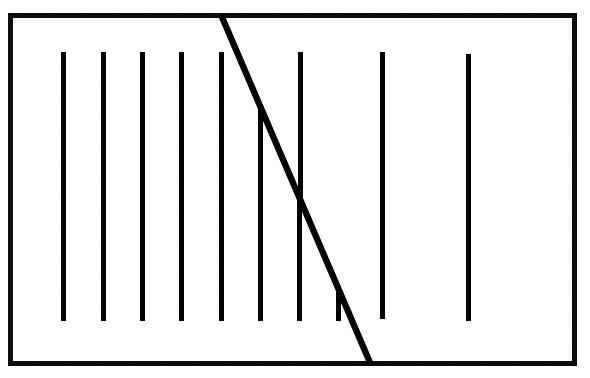
\includegraphics[width=.3\textwidth]{./img/ch2_weekend_mc_2024-05-31-18-33-30.png}\par}
        \task \topalign{\par\centering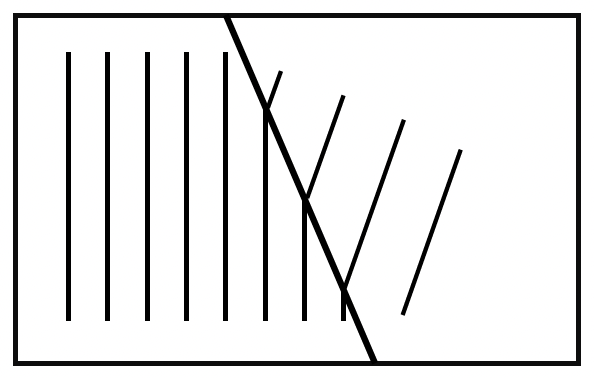
\includegraphics[width=.3\textwidth]{./img/ch2_weekend_mc_2024-05-31-18-33-45.png}\par}
        \task \topalign{\par\centering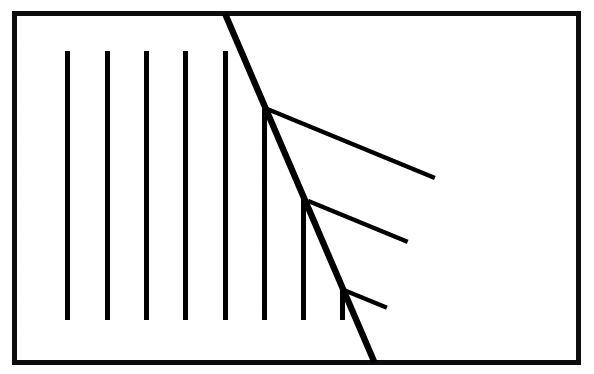
\includegraphics[width=.3\textwidth]{./img/ch2_weekend_mc_2024-05-31-18-34-08.png}\par}
        \task \topalign{\par\centering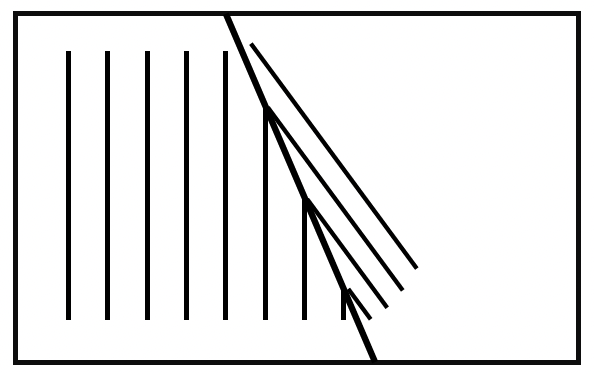
\includegraphics[width=.3\textwidth]{./img/ch2_weekend_mc_2024-05-31-18-33-57.png}\par}
    \end{tasks}
}{B}

% \newprob{1717151812}
% {
%     % q18 cancelled because its superposition
%     一列正弦水波向牆壁傳播,圖示一刻是水波剛抵達牆壁的瞬間。$P$ 是一個浮在水面的粒子,它的
%     初始位置接近牆壁。\\A sinusoidal water wave is propagating towards a wall. The diagram represents a moment when the water wave has just reached the wall. $P$ is a particle floating on the water surface, initially positioned near the wall.
%     \par{\par\centering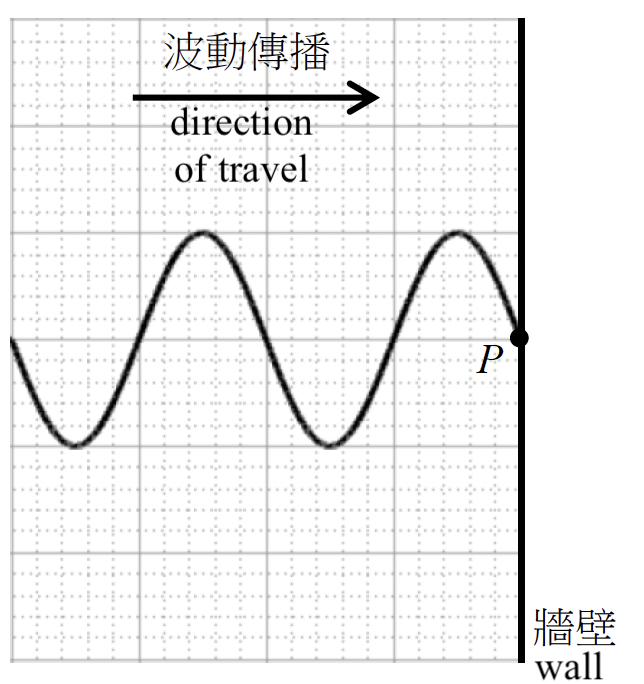
\includegraphics[width=.3\textwidth]{./img/ch2_weekend_mc_2024-05-31-18-40-31.png}\par}
%     已知水波的振幅是 1 cm。在四分之一個週期後,P 從平衡位置的位移量值是多少?\\The amplitude of the water wave is known to be 1 cm. After one-quarter of a period, what is the magnitude of displacement of P from its equilibrium position?
%     \begin{tasks}
%         \task 2 cm
%         \task $\sqrt{2}$ cm
%         \task 1 cm
%         \task 0 cm
%     \end{tasks}
% }{}

\newprob{1717152111}
{
    % 模考前功課二 q23
    防波堤是海邊的一種人造結構,目的是抵擋海浪。\\A breakwater is a man-made structure located at the seaside, designed to resist the impact of ocean waves.
    \par{\par\centering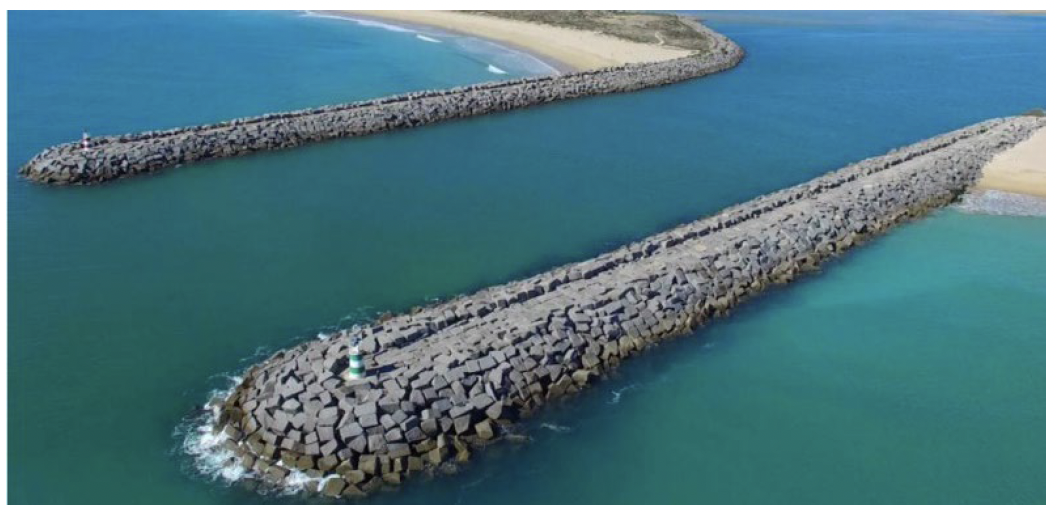
\includegraphics[width=.45\textwidth]{./img/ch2_weekend_mc_2024-05-31-18-44-09.png}\par}
    \par{\par\centering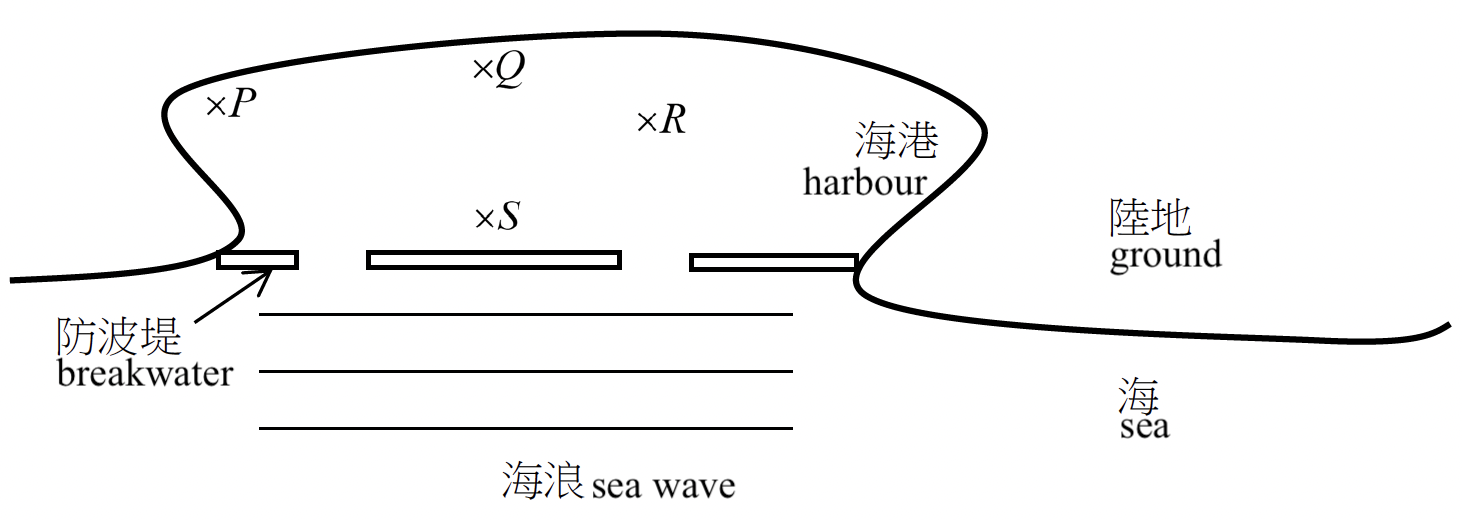
\includegraphics[width=.45\textwidth]{./img/ch2_weekend_mc_2024-05-31-18-45-31.png}\par}
    一艘船停泊在海港中。圖中四個標示的位置中,何者受到海浪影響的可能性最小?\\Among the four labeled positions shown in the diagram, which one is least likely to be affected by ocean waves?
    \begin{tasks}
        \task $P$
        \task $Q$
        \task $R$
        \task $S$
    \end{tasks}

}{D}

\newprob{1717152636}
{
    某次海底地震產生了海嘯(海嘯可視為巨大的水波)。一艘船與發生地震的位置的水平距離是20
    km,這艘船上的船員幾乎感覺不到海嘯的經過,但這海嘯卻嚴重影響1200 km 遠的小島。下列何
    者是最佳解釋?\\The occurrence of an underwater earthquake generated a tsunami (which can be seen as a massive water wave). A ship is located 20 km horizontally away from the epicenter of the earthquake. The crew on the ship hardly feels the passage of the tsunami. However, this tsunami severely affects a small island located 1200 km away. Which of the following is the best explanation?
    \par{\par\centering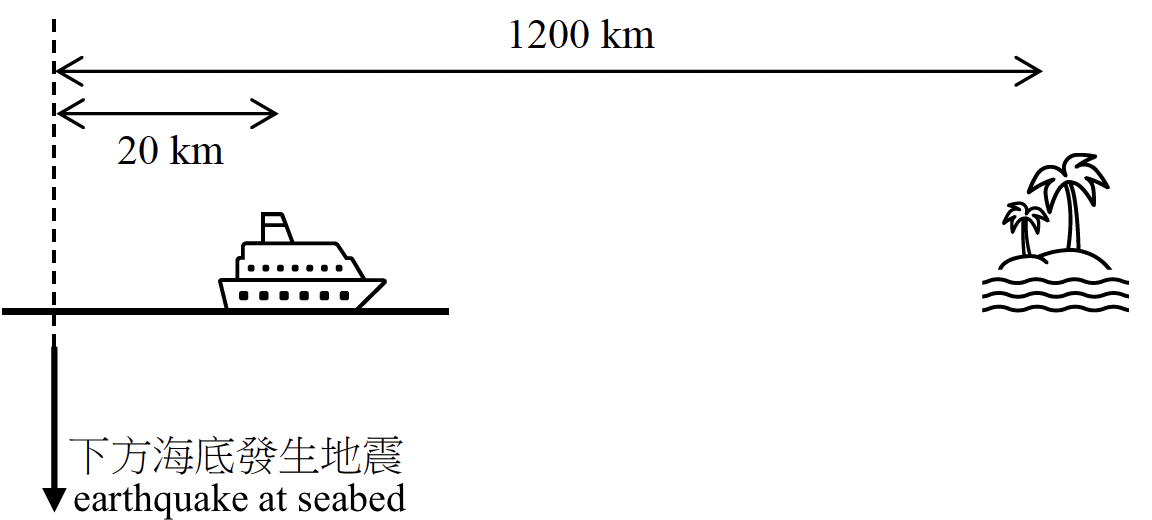
\includegraphics[width=.5\textwidth]{./img/ch2_weekend_mc_2024-05-31-18-52-07.png}\par}
    \begin{tasks}
        \task 海嘯傳播期間,頻率持續下降。\\During the propagation of a tsunami, the frequency continues to decrease.
        \task 海嘯傳播越遠,它的振幅越大。\\The further a tsunami propagates, the greater its amplitude.
        \task 海嘯是一種機械波。\\A tsunami is a mechanical wave.
        \task 船所在的位置水波波速遠高於抵達小島時的波速。\\The wave speed at the location of the boat is much higher than the wave speed when it reaches the small island.
    \end{tasks}

}{D}

\newprob{1717153384}
{
    A straight sound wave propagates to the right. After passing through region X, the wavefront changes into an arc shape, as shown in the diagram.\\一列直線聲波向右傳播,經過區域X後,波陣面變成圓弧形,如圖所示。
    \par{\par\centering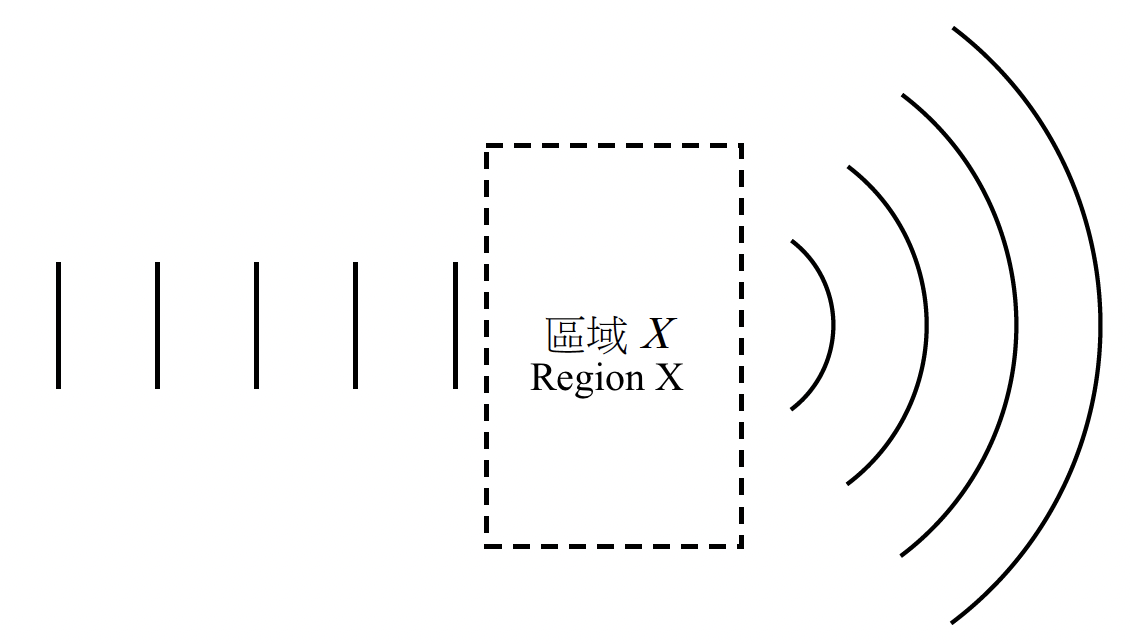
\includegraphics[width=.5\textwidth]{./img/ch2_weekend_mc_2024-05-31-19-03-39.png}\par}
    下列哪些可能是區域X中的設置?\\Which of the following can be the setup in X?
    \begin{statements}
        \task \topalign{\par\centering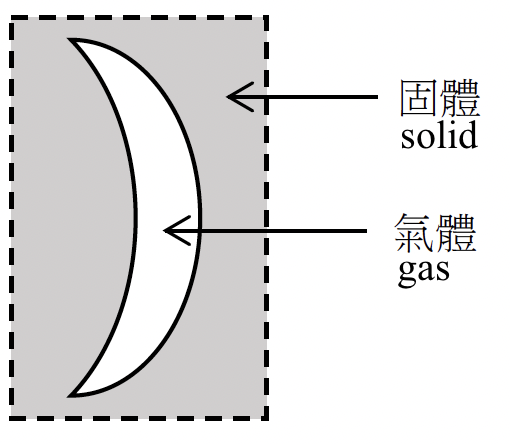
\includegraphics[width=.2\textwidth]{./img/ch2_weekend_mc_2024-05-31-19-05-30.png}\par}
        \task \topalign{\par\centering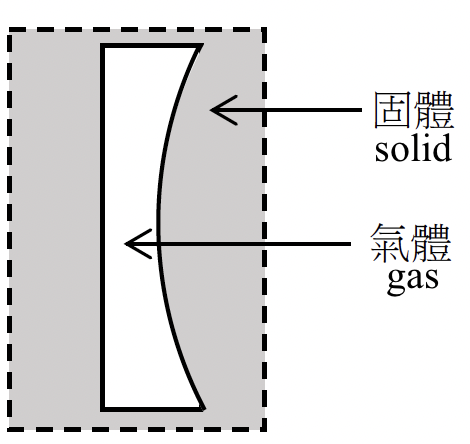
\includegraphics[width=.2\textwidth]{./img/ch2_weekend_mc_2024-05-31-19-06-03.png}\par}
        \task \topalign{\par\centering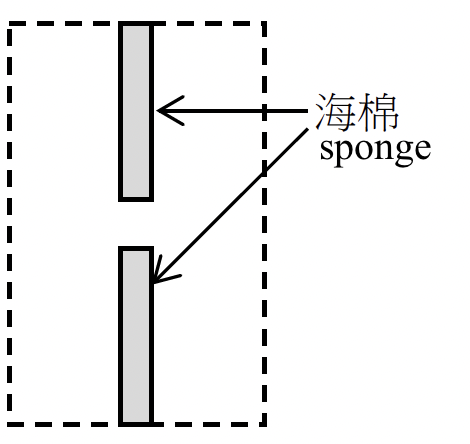
\includegraphics[width=.2\textwidth]{./img/ch2_weekend_mc_2024-05-31-19-06-28.png}\par}
    \end{statements}

    \begin{tasks}
        \task 只有(1) \tab\tab  (1) only
        \task 只有(2) \tab\tab  (2) only
        \task 只有(1)和(3) \tab\tab  (1) and (3) only
        \task 只有(2)和(3) \tab \tab (2) and (3) only
    \end{tasks}
}{C}

\newprob{1717153704}
{
    在一個門敞開的教室中,Steve 打開嗓門在開罵。教室外的李同學在圖示位置聽到 Steve 的聲音。\\In an open classroom with the door ajar, Steve starts shouting. Mr. Li, a student outside the classroom, hears Steve's voice at the indicated location in the diagram.
    \par{\par\centering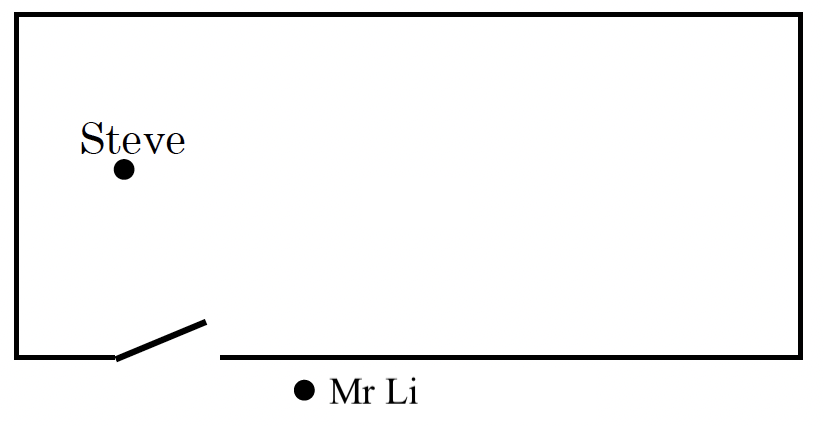
\includegraphics[width=.4\textwidth]{./img/ch2_weekend_mc_2024-05-31-19-11-06.png}\par}
    李同學與Steve之間雖然有門和牆壁遮擋,但仍然聽到他的聲音。下列哪個現象最能解釋這現象?\\Despite the presence of doors and walls between Li and Steve, Li can still hear Steve's voice. Which phenonmenon best explains the situation?
    \begin{tasks}
        \task 反射 reflection
        \task 折射 refraction
        \task 衍射 diffraction
        \task 以上都是 All of the above
    \end{tasks}

}{C}

\newprob{1717154175}
{
    李同學雖聽到聲音但看不見Steve。下列何者是最佳解釋?\\Mr Li can hear the voice but can't see Steve, which of the following best explains the phenonmenon?
    \begin{tasks}
        \task 光的速率遠比聲音高。\\Speed of light is faster than speed of sound.
        \task 光的波長遠比聲音短。\\Wavelength of light is shorter than wavelength of sound.
        \task 光是橫波但聲音是縱波。\\Light is transverse wave but sound is longitudinal wave
        \task 只有波動才可繞過障礙物。\\Only wave can diffract around obstacles.
    \end{tasks}
}{B}